\documentclass[10pt,letterpaper]{article}

\usepackage{fontspec}
\setmainfont{texgyretermes-regular.otf}[BoldFont=texgyretermes-bold.otf,ItalicFont=texgyretermes-italic.otf,BoldItalicFont=texgyretermes-bolditalic.otf]
\usepackage{unicode-math}
\setmathfont{texgyretermes-math.otf}

\usepackage[letterpaper,margin=1in]{geometry}
\usepackage{amsmath}
\usepackage{graphicx}
\usepackage{booktabs}
\usepackage{array}
\usepackage{tabularx}
\usepackage[font=small,labelfont=bf,justification=raggedright,singlelinecheck=false]{caption}
\usepackage{microtype}
\usepackage[hidelinks]{hyperref}
\hypersetup{
  pdftitle={Zero Resistance, Zero Speedup: A Room-Temperature Superconductor Would Change Interconnect Reach, Not Latency},
  pdfauthor={Amrendra Singh and DeepSeek V4.1 Flash 1017},
  pdfsubject={superconductivity, interconnect, data links, cryogenics},
  pdfkeywords={superconductor, interconnect, kinetic inductance, cryocooler, data link}
}
\usepackage{titlesec}

\graphicspath{{../figures/}}

\setlength{\parindent}{1.2em}
\setlength{\parskip}{0pt}
\emergencystretch=1em

\titleformat{\section}{\large\bfseries}{\thesection.}{0.5em}{}
\titleformat{\subsection}{\normalsize\bfseries}{\thesubsection}{0.5em}{}
\titlespacing*{\section}{0pt}{1.5ex plus .3ex}{0.6ex}
\titlespacing*{\subsection}{0pt}{1.2ex plus .2ex}{0.3ex}

\begin{document}

\title{\textsc{\small Technical Report $\cdot$ Position Paper}\\[10pt]
\textbf{Zero Resistance, Zero Speedup}\\[5pt]
{\large A Room-Temperature Superconductor Would Change Interconnect Reach, Not Latency}}
\author{\normalsize Amrendra Singh and DeepSeek V4.1 Flash 1017}
\date{\normalsize 2026}
\maketitle
\vspace{-1.4em}

\begin{abstract}
\noindent Superconductivity is the most seductive material promise in computing: a wire with no resistance, carrying data at the speed of light, losing nothing. This position paper argues that the promise is real but misdirected. A superconductor removes DC resistance; it does not remove the driver, the receiver, the package, the connector, or the protocol. At gigahertz frequencies a superconducting line is an LC transmission line with kinetic inductance, and its propagation delay can be longer than copper's. The energy and latency of a link are dominated by the last centimeter---the CMOS interface---not by the wire. Using a first-order link model, we show that zero resistance moves the crossover between electrical and optical links by orders of magnitude in reach, not by a factor in latency. We state the status of the field plainly: no ambient-pressure room-temperature superconductor has been verified; the claims that reached room temperature required megabar pressures or failed replication. We then treat a manufacturable room-temperature superconductor as a hypothesis and derive what would have to be true for it to matter. The answer is a research agenda: measure energy per bit per meter at 300 K, not resistance at 4 K.
\end{abstract}

\noindent\textbf{Keywords:} superconductivity; interconnect; kinetic inductance; cryocooler; data link; memory bandwidth.

\section{Introduction}
\label{sec:intro}

Every few years a material arrives that seems to dissolve a law of economics. Room-temperature superconductivity is the current candidate. A wire with no resistance would carry current without loss, at any distance, with no cooling. The intuition is that data would then travel faster, farther, and cheaper, and that the interconnect problem would be solved.

The intuition is half right, and the half that is wrong is the half that matters. Data in a computer is already carried by electricity: voltage and current in copper, modulated by a driver and recovered by a receiver. A superconductor changes the properties of the wire, not the properties of the driver, the receiver, the package, the connector, or the protocol. Those components set the latency and the energy of a link, and they are made of semiconductors, not superconductors. The wire is a passive middleman.

This paper makes a position argument: a room-temperature superconductor would be a reach technology, not a latency technology. It would let a link span meters instead of centimeters at low loss, and it would remove the cryogenic plant that confines today's superconducting links to quantum and SFQ systems. It would not make a cache-line fetch faster, because the fetch is dominated by the protocol round trip, not by the time a bit spends on the wire. And it would not remove the last centimeter---the CMOS interface---where the energy and the latency are actually spent.

Our contributions are four. First, we separate what superconductivity does to a link from what it does not (Section~\ref{sec:physics}). Second, we decompose the latency and energy of a link and show that the wire is a minority of both (Section~\ref{sec:lastcm}). Third, we build a first-order model of energy per bit as a function of length and temperature, and derive the crossover length at which a superconducting link beats copper (Section~\ref{sec:economics}). Fourth, we treat a manufacturable room-temperature superconductor as a hypothesis, state the material properties it would need, and identify where it would win first (Sections~\ref{sec:changes} and~\ref{sec:wins}).

We owe the reader a plain statement of the field's status.\footnote{Status as of early 2026. Primary claims and retractions are cited in the references.} As of 2026, no ambient-pressure room-temperature superconductor has been verified. The highest accepted transition temperature at ambient pressure is about 150~K in mercury cuprates \cite{schilling}; the highest at high pressure is about 250~K in lanthanum decahydride at roughly 150~GPa \cite{drozdov2019}. The 2020 carbonaceous sulfur hydride claim (288~K at 267~GPa) was retracted \cite{snider,sniderretract}; the 2023 nitrogen-doped lutetium hydride claim (294~K at 1~GPa) failed replication and was retracted \cite{dasenbrock,dasenbrockretract}; LK-99 was shown not to be a superconductor \cite{lk99}. None of this diminishes the field. It defines the gap between a diamond-anvil sample and a manufacturable cable, which is the subject of this paper.

\section{What Superconductivity Does to a Link}
\label{sec:physics}

\subsection{Zero DC resistance, finite AC resistance}

A superconductor below its critical temperature has zero DC resistance. That is the property that makes magnets, power cables, and SQUIDs possible \cite{tinkham}. A data link, however, does not carry DC. It carries a modulated signal whose spectrum extends from a few gigahertz to tens of gigahertz. At those frequencies the relevant quantity is the surface resistance $R_s$, not the DC resistance. For a clean s-wave superconductor well below the gap, $R_s \propto \omega^2$; at 4~K and 10~GHz it can be orders of magnitude below copper's surface resistance, but it is not zero. At 77~K the quasiparticle population is larger and $R_s$ is higher; at 300~K, if a room-temperature superconductor exists, $R_s$ is higher still. The wire is low-loss, not lossless \cite{pozar}.

\subsection{Kinetic inductance makes the wire slower}

The supercurrent has inertia. The kinetic inductance of a film is
\begin{equation}
L_k = \frac{m}{n_s e^2 A},
\end{equation}
where $n_s$ is the superfluid density and $A$ is the cross-section. In a thin film, $L_k$ can exceed the magnetic inductance $L_m$. The propagation velocity of a superconducting transmission line is
\begin{equation}
v = \frac{1}{\sqrt{(L_k+L_m)C}},
\end{equation}
which is lower than the geometric $1/\sqrt{L_m C}$. For a 50~nm YBCO strip, $L_k$ can dominate, and $v$ can fall to 0.1--0.5$c$. The characteristic impedance
\begin{equation}
Z_0 = \sqrt{\frac{L_k+L_m}{C}}
\end{equation}
can be far below 50~$\Omega$, which makes the driver's job harder, not easier. This is the first counterintuitive result of the paper: a superconductor can be slower than copper.

\subsection{Critical current, quench, and noise}

The price of zero resistance is a critical current $J_c$ and a critical field $H_{c2}$. A data link carries little average current, but the driver must charge the line capacitance on every edge; the peak current can be large. A defect that drives the line normal can quench it, dumping the stored magnetic energy into a small volume. Vortex motion produces phase noise, which becomes bit-error rate. None of these problems is fatal, but each is a reason why a superconducting link is a system, not a wire.

\subsection{Material families}

Table~\ref{tab:materials} separates the field into three tiers. The first tier is mature: niobium, niobium nitride, magnesium diboride, and the cuprates, all at ambient pressure, with $T_c$ from 9 to 110~K \cite{bednorz,wu}. The second tier is high-pressure hydrides: H$_3$S at 203~K and LaH$_{10}$ at 250~K, both at roughly 150~GPa \cite{drozdov2015,somayazulu,drozdov2019}. The third tier is the room-temperature claims: carbonaceous sulfur hydride (288~K at 267~GPa, retracted), nitrogen-doped lutetium hydride (294~K at 1~GPa, retracted and unreplicated), and LK-99 (claimed 400~K at ambient pressure, shown not to be a superconductor). A room-temperature superconductor would be a fourth tier. The rest of this paper asks what that tier would change.

\begin{table}[t]
\centering
\caption{Superconductor families relevant to interconnects. The first tier is commercially available; the second requires megabar pressures; the third consists of claims that failed replication.}
\label{tab:materials}
\small
\begin{tabularx}{\linewidth}{@{}lccX@{}}
\toprule
Family & $T_c$ (K) & Pressure & Status and typical use \\
\midrule
Nb & 9.3 & 1 atm & Mature; 4 K; SFQ logic, MRI, accelerator magnets \\
NbN & 16 & 1 atm & Mature; 4 K; detectors, digital circuits \\
MgB$_2$ & 39 & 1 atm & Mature; 20 K; wires, magnets \\
YBCO & 92 & 1 atm & Commercial coated conductors; 77 K; power cables, magnets \\
BSCCO & 110 & 1 atm & Commercial tapes; 77 K; power cables \\
Hg-1223 & 133--151 & 1 atm & Lab; highest ambient-pressure $T_c$ \\
H$_3$S & 203 & $\sim$150 GPa & Lab; high-pressure hydride \\
LaH$_{10}$ & 250 & $\sim$150 GPa & Lab; highest accepted $T_c$ \\
CSH & 288 & 267 GPa & Retracted (2022); room-temperature claim \\
LuNH & 294 & 1 GPa & Retracted; replication failed \\
LK-99 & 400 (claimed) & 1 atm & Not a superconductor (2023) \\
\bottomrule
\end{tabularx}
\end{table}

\section{The Last Centimeter}
\label{sec:lastcm}

\subsection{The stack}

A link is not a wire. It is a chain: a CMOS driver, a bump, a package trace, a connector, a cable, a second connector, a second package, a second bump, and a CMOS receiver. The superconductor replaces the cable and, at best, the package trace. The driver, the receiver, the bumps, and the connectors remain. Each interface is a discontinuity with capacitance, inductance, and loss. At 10~GHz, a connector can cost more signal integrity than a meter of cable.

\subsection{Latency}

The latency of a link is
\begin{equation}
t_{\mathrm{link}} = t_{\mathrm{tx}} + t_{\mathrm{wire}} + t_{\mathrm{rx}} + t_{\mathrm{serdes}} + t_{\mathrm{protocol}}.
\end{equation}
For a 1~m link, $t_{\mathrm{tx}} \approx t_{\mathrm{rx}} \approx 20$~ps, $t_{\mathrm{wire}} \approx 6.7$~ns in copper (0.5$c$) or 11.1~ns in a superconductor with $v=0.3c$, $t_{\mathrm{serdes}} \approx 100$~ps, and $t_{\mathrm{protocol}} \approx 500$~ns for a PCIe round trip \cite{pcie6}. The wire is 1--2\% of the total. A superconductor that made the wire infinitely fast would save at most 11~ns, or 2\% of the round trip. Figure~\ref{fig:latency} shows the budget on a log scale; the protocol bar is two orders of magnitude longer than the wire bar.

\begin{figure}[t]
\centering
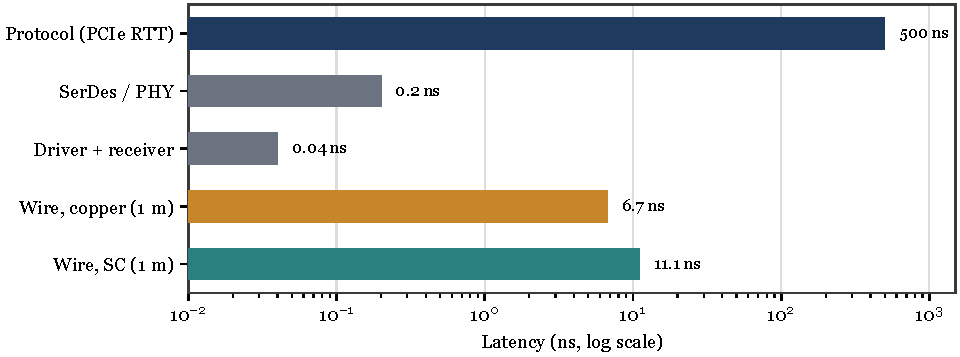
\includegraphics[width=\linewidth]{fig2_latency.pdf}
\caption{Latency budget of a 1~m link, on a log scale. The protocol round trip dominates by two orders of magnitude; the wire, superconducting or not, is a rounding error.}
\label{fig:latency}
\end{figure}

\subsection{Energy}

The energy per bit is
\begin{equation}
E_b = E_{\mathrm{tx}} + E_{\mathrm{wire}} + E_{\mathrm{rx}} + E_{\mathrm{clock}}.
\end{equation}
At 32~Gb/s in a 7~nm CMOS SerDes, $E_{\mathrm{tx}} \approx E_{\mathrm{rx}} \approx 150$~fJ/bit and $E_{\mathrm{clock}} \approx 100$~fJ/bit \cite{horowitz}. Optical links have a different energy budget, but the same lesson: the interface, not the medium, sets the floor \cite{miller}. A copper trace at 16~GHz loses roughly 0.5--1~dB per inch, so a 1~m link costs on the order of 2~pJ/bit in wire loss; a superconducting cable with $R_s$ two orders of magnitude lower costs about 0.01~pJ/bit/m. At 1~m, copper totals about 2.4~pJ/bit and a superconductor about 0.4~pJ/bit, a 6$\times$ saving. At 0.1~m, copper totals about 0.6~pJ/bit and a superconductor about 0.4~pJ/bit, a 1.5$\times$ saving. The wire matters at 1~m; the interface matters at 0.1~m. Figure~\ref{fig:breakdown} shows both.

\begin{figure}[t]
\centering
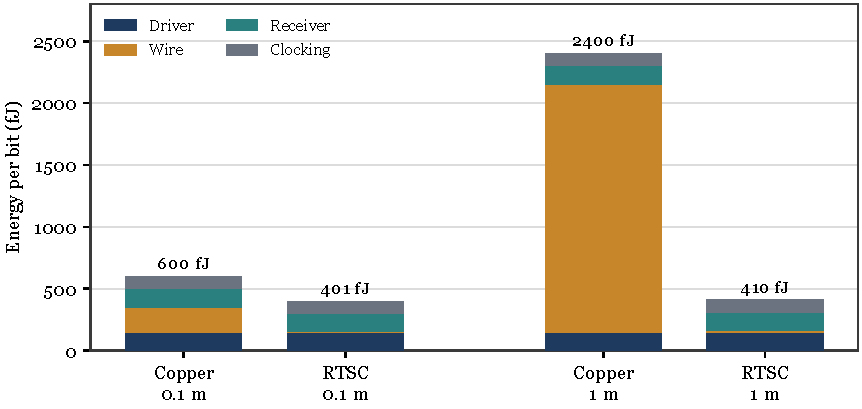
\includegraphics[width=\linewidth]{fig4_energy_breakdown.pdf}
\caption{Energy per bit at 0.1~m and 1~m, decomposed into driver, wire, receiver, and clocking. At 0.1~m the interface dominates for both technologies; at 1~m the copper wire dominates and the superconductor removes it.}
\label{fig:breakdown}
\end{figure}

\subsection{The last centimeter}

The last centimeter is the driver, the bump, the package, the connector, and the receiver. It is where the energy is spent at short reach and where the reflections are generated at any reach. A superconducting cable with copper connectors is a chain of losses; the connectors can dominate the link. A room-temperature superconductor does not change this, because the connectors are not superconducting. The last centimeter is the real bottleneck, and it is a packaging problem, not a materials problem.

\section{The Economics of Zero Resistance}
\label{sec:economics}

\subsection{Model}

Let $E_0 = E_{\mathrm{tx}} + E_{\mathrm{rx}}$ be the fixed interface energy, $\alpha$ the wire energy per bit per meter, and $\eta(T)$ the cryogenic overhead, defined as the ratio of room-temperature power to the heat removed at temperature $T$. For a superconducting link,
\begin{equation}
E_b(L,T) = \bigl(1+\eta(T)\bigr)\bigl(E_0 + \alpha_{\mathrm{sc}} L\bigr),
\end{equation}
and for copper at 300~K,
\begin{equation}
E_b(L,300) = E_0 + \alpha_{\mathrm{cu}} L.
\end{equation}
The cryogenic overhead multiplies the whole link, not just the wire: the driver and receiver also dissipate at the cold stage. This is the key asymmetry.

\subsection{Cryogenic overhead}

At 4~K, a practical cryocooler removes about 1~W for every 300~W of input, so $\eta \approx 300$; at 77~K the ratio is about 1:20, so $\eta \approx 20$; at 300~K, $\eta = 0$ \cite{radebaugh}. These are order-of-magnitude numbers; the point is that the overhead is a multiplier, not an addend.

\subsection{Crossover length}

Set the two energies equal and solve for $L$:
\begin{equation}
L^* = \frac{\eta E_0}{\alpha_{\mathrm{cu}} - (1+\eta)\alpha_{\mathrm{sc}}}.
\end{equation}
With $E_0 = 300$~fJ, $\alpha_{\mathrm{cu}} = 2$~pJ/bit/m, and $\alpha_{\mathrm{sc}} = 0.01$~pJ/bit/m, the crossover is 3.3~m at 77~K and does not exist at 4~K: the denominator is negative, so the superconducting link never beats copper. At 300~K, $\eta = 0$ and $L^* = 0$: the superconducting link wins at any length, by 1.99~pJ/bit/m. Figure~\ref{fig:energy} plots the energy versus length; Figure~\ref{fig:crossover} plots the crossover versus $\eta$.

The shape is the message. At 4~K, the cryogenic overhead dominates and the link is only viable inside a cryostat that is already paid for. At 77~K, the link wins beyond a few meters, which is a backplane, not a chip-to-chip link. At 300~K, the link wins everywhere, but the absolute saving at 0.1~m is 0.1~pJ/bit, which is small compared with the CMOS energy.

\begin{figure}[t]
\centering
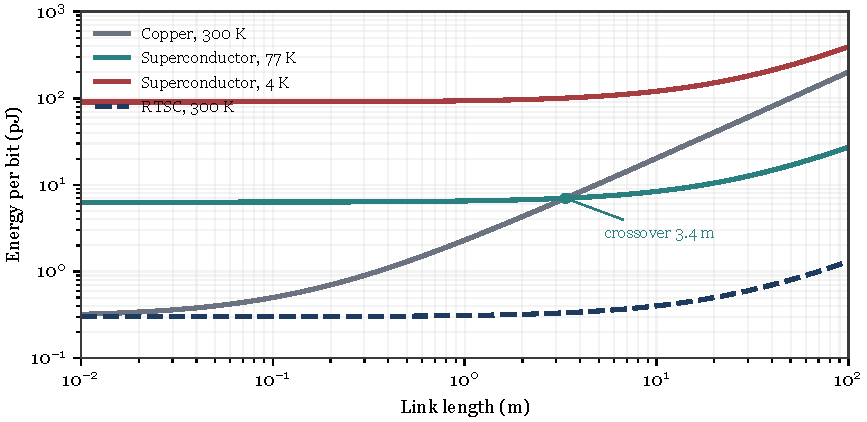
\includegraphics[width=\linewidth]{fig1_energy_length.pdf}
\caption{Energy per bit versus link length. The cryogenic overhead is a multiplier, so the 4~K link never beats copper for data. The 77~K link wins beyond about 3~m. The room-temperature superconductor wins everywhere, but the absolute saving at short reach is small.}
\label{fig:energy}
\end{figure}

\begin{figure}[t]
\centering
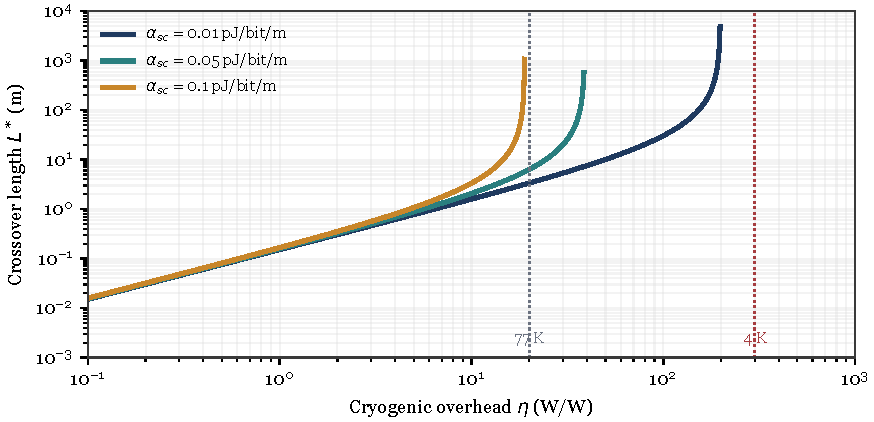
\includegraphics[width=\linewidth]{fig3_crossover.pdf}
\caption{Crossover length versus cryogenic overhead, for three values of the superconducting wire loss. The vertical lines mark 77~K and 4~K. At 4~K, no positive crossover exists for these parameters: the cryogenic overhead is larger than the wire loss it removes.}
\label{fig:crossover}
\end{figure}

\subsection{What the model does not say}

The model is first-order. It ignores the temperature dependence of $R_s$, the frequency dependence of the dielectric loss, the connector loss, the driver's impedance matching, and the cost of the cryostat. It assumes that the superconducting line has the same capacitance as copper, which is optimistic for a thin-film line with high kinetic inductance. It assumes that the cryocooler's COP is constant, which is optimistic at 4~K. The conclusion is robust to these approximations because the gap is orders of magnitude, not a few percent.

\section{What a Room-Temperature Superconductor Would Change}
\label{sec:changes}

\subsection{What changes}

A room-temperature superconductor removes the cryogenic plant. That is the largest system-level change: no liquid helium, no vacuum vessel, no cold finger, no multi-stage cooler. It enables flexible, bendable, high-density cables; it allows longer reach without repeaters; it reduces the link's energy at long lengths; and it makes superconducting power delivery practical. Table~\ref{tab:changes} lists the changes.

\subsection{What does not change}

The CMOS driver and receiver still dominate at short reach. The package, the connector, and the via are still copper, still lossy, still reflective. The protocol still has a round trip of hundreds of nanoseconds, still has tags and credits, still moves 64-byte cache lines. The memory hierarchy still has capacity, banks, and latency. The economics still has cost per meter, yield, test, and repair. A room-temperature superconductor changes the wire; it does not change the system around the wire.

\begin{table}[t]
\centering
\caption{A room-temperature superconductor changes the wire, not the system around it.}
\label{tab:changes}
\small
\begin{tabularx}{\linewidth}{@{}XX@{}}
\toprule
Changes & Does not change \\
\midrule
Cryogenic plant (removed) & CMOS driver and receiver energy \\
Reach (meters to kilometers) & Package, connector, and via loss \\
Wire loss (lower) & Protocol round trip, tags, credits \\
Cable flexibility and density & Memory capacity, banks, latency \\
Power delivery (zero $I^2R$) & Cost, yield, test, repair \\
\bottomrule
\end{tabularx}
\end{table}

\subsection{The material requirements}

For a superconductor to matter as a data link at 300~K, it needs more than $T_c > 300$~K. It needs a critical current density above $10^7$~A/cm$^2$ in self-field, a surface resistance below 1~m$\Omega$ at 10~GHz, a critical field above 10~T for power applications, a bend radius below 1~cm, strain tolerance above 1\%, a CMOS-compatible process, a cost below \$1/m, and a yield above 90\%. Table~\ref{tab:targets} compares these targets with the current state. The gap is not one number; it is a stack of them.

\begin{table}[t]
\centering
\caption{Material targets for a room-temperature interconnect, compared with the current state.}
\label{tab:targets}
\small
\begin{tabularx}{\linewidth}{@{}lXX@{}}
\toprule
Metric & Target & Current state \\
\midrule
$T_c$ at 1 atm & $>300$~K & $\sim$150~K (Hg-1223); 250~K at 150~GPa (LaH$_{10}$) \\
$J_c$ at 300~K, self-field & $>10^7$~A/cm$^2$ & $\sim10^6$~A/cm$^2$ (YBCO films at 77~K) \\
$R_s$ at 10~GHz, 300~K & $<1$~m$\Omega$ & $\sim1$~m$\Omega$ (Nb at 4~K) \\
Pressure & 1~atm & 150~GPa (LaH$_{10}$) \\
Bend radius & $<1$~cm & 1--10~cm (coated conductors) \\
CMOS compatibility & Yes & No (epitaxy or pressure) \\
Cost & $<\$1$/m & \$10--100/m (YBCO tape) \\
Yield & $>90\%$ & Lab-scale \\
\bottomrule
\end{tabularx}
\end{table}

\subsection{The last centimeter remains}

Even a perfect superconductor has to connect to a copper bump, a copper package, and a copper connector. The contact resistance, the inductance of the bump, and the impedance discontinuity of the connector remain. The driver must charge the line capacitance; a low-$Z_0$ superconducting line is harder to drive, not easier. The receiver must amplify a small signal; the SNR is set by the driver and the channel, not by the wire's resistance. The last centimeter is where the link is won or lost.

\section{Where It Wins First}
\label{sec:wins}

\subsection{Power delivery}

The first application is not data; it is power. A zero-resistance cable can carry current without $I^2R$ loss, which is a transmission-line problem with different requirements: high current, low voltage, and AC loss at 50--60~Hz. A room-temperature superconductor would change grid and datacenter power distribution before it changes a memory bus.

\subsection{Cryogenic systems}

Quantum computers, SFQ logic, and superconducting detectors already pay for the cryogenic plant. Inside that plant, the marginal cost of a superconducting link is low, and the link's heat load is the price of admission. This is where superconducting links are used today, and where they will continue to win \cite{likharev,holmes,monroe}.

\subsection{Long-haul and backplanes}

If flexible room-temperature cables exist, the first data application is the backplane: 1--10~m, high density, low loss. The connector is the challenge. A superconducting cable with copper connectors is only as good as its connectors, and a backplane has many of them.

\subsection{Not cache-line memory}

The memory link is short (centimeters), latency-sensitive, and protocol-bound. A superconductor saves 6.7~ns/m; the protocol is 500~ns; the tag space is 256; the payload is 64~B. The bottleneck is concurrency, not resistance \cite{pcie6,cxl}. A superconductor does not add tags, pins, or payload size. It does not make a cache-line fetch faster.

\section{A Research Agenda}
\label{sec:agenda}

\subsection{Metrics}

The field needs a metric that matches the application: energy per bit per meter at 300~K, latency per meter at 300~K, critical current at 300~K in self-field, surface resistance at 10~GHz and 300~K, bend radius, strain tolerance, cost per meter, and yield. Resistance at 4~K is not the metric.

\subsection{Material targets}

Table~\ref{tab:targets} lists the targets. The most important are $J_c > 10^7$~A/cm$^2$, $R_s < 1$~m$\Omega$ at 10~GHz, $T_c > 300$~K at ambient pressure, a bend radius below 1~cm, and a CMOS-compatible process. A material that meets $T_c$ but not $J_c$ is a science result, not an interconnect.

\subsection{System targets}

A 1~Tb/s link over 1~m at less than 1~pJ/bit, with less than 1~ns of added latency, 1,000 bending cycles, and a 10-year lifetime. These are the numbers that a system designer would recognize \cite{irds}.

\subsection{What would change our mind}

A verified ambient-pressure room-temperature superconductor with $J_c > 10^7$~A/cm$^2$ and $R_s < 1$~m$\Omega$ at 10~GHz; a demonstrated 1~Tb/s superconducting cable with copper connectors; a CMOS-compatible process; and a cost model below \$1/m. Until then, the room-temperature superconductor is a hypothesis, and the paper's argument is conditional.

\section{Conclusion}
\label{sec:conclusion}

Zero resistance is a means, not an end. The end is moving a bit from one place to another with the least energy and the least delay. A superconductor removes one term from that budget---the wire's resistance---and leaves the others: the driver, the receiver, the package, the connector, the protocol. A room-temperature superconductor would be a genuine breakthrough, but its first consequence for computing would be reach, not speed. It would let us build longer, denser, lower-loss electrical links, and it would remove the cryogenic plant that confines superconducting links to specialized systems. It would not make a cache-line fetch faster, because the fetch is dominated by the protocol round trip. The right question is not ``how fast is the superconductor?'' but ``how far can we afford to move a bit?'' For the next decade, the answer is still: not far enough.

\begingroup
\raggedright
\begin{thebibliography}{99}

\bibitem{bednorz} J. G. Bednorz and K. A. Müller, ``Possible high $T_c$ superconductivity in the Ba--La--Cu--O system,'' \emph{Zeitschrift für Physik B}, vol. 64, pp. 189--193, 1986.

\bibitem{wu} M. K. Wu, J. R. Ashburn, C. J. Torng, \emph{et al.}, ``Superconductivity at 93 K in a new mixed-phase Y--Ba--Cu--O compound system at ambient pressure,'' \emph{Physical Review Letters}, vol. 58, pp. 908--910, 1987.

\bibitem{schilling} A. Schilling, M. Cantoni, J. D. Guo, and H. R. Ott, ``Superconductivity above 130 K in the Hg--Ba--Ca--Cu--O system,'' \emph{Nature}, vol. 363, pp. 56--58, 1993.

\bibitem{drozdov2015} A. P. Drozdov, M. I. Eremets, I. A. Troyan, V. Ksenofontov, and S. I. Shylin, ``Conventional superconductivity at 203 kelvin at high pressures in the sulfur hydride system,'' \emph{Nature}, vol. 525, pp. 73--76, 2015.

\bibitem{somayazulu} M. Somayazulu, M. Ahart, A. K. Mishra, \emph{et al.}, ``Evidence for superconductivity above 260 K in lanthanum superhydride at megabar pressures,'' \emph{Physical Review Letters}, vol. 122, 027001, 2019.

\bibitem{drozdov2019} A. P. Drozdov, P. P. Kong, V. S. Minkov, \emph{et al.}, ``Superconductivity at 250 K in lanthanum hydride under high pressures,'' \emph{Nature}, vol. 569, pp. 528--531, 2019.

\bibitem{snider} E. Snider, N. Dasenbrock-Gammon, R. McBride, \emph{et al.}, ``Room-temperature superconductivity in a carbonaceous sulfur hydride,'' \emph{Nature}, vol. 586, pp. 373--377, 2020.

\bibitem{sniderretract} ``Retraction Note: Room-temperature superconductivity in a carbonaceous sulfur hydride,'' \emph{Nature}, vol. 610, p. 804, 2022.

\bibitem{dasenbrock} N. Dasenbrock-Gammon, E. Snider, R. McBride, \emph{et al.}, ``Evidence of near-ambient superconductivity in a N-doped lutetium hydride,'' \emph{Nature}, vol. 615, pp. 244--250, 2023.

\bibitem{dasenbrockretract} ``Retraction Note: Evidence of near-ambient superconductivity in a N-doped lutetium hydride,'' \emph{Nature}, vol. 623, p. 1005, 2023.

\bibitem{lk99} S. Lee, J.-H. Kim, and Y.-W. Kwon, ``The first room-temperature ambient-pressure superconductor,'' arXiv:2307.12008, 2023; see also the replication reports of 2023.

\bibitem{tinkham} M. Tinkham, \emph{Introduction to Superconductivity}, 2nd ed. New York: McGraw-Hill, 1996.

\bibitem{pozar} D. M. Pozar, \emph{Microwave Engineering}, 4th ed. Hoboken, NJ: Wiley, 2011.

\bibitem{radebaugh} R. Radebaugh, ``Cryocoolers: the state of the art and recent developments,'' \emph{Journal of Physics: Condensed Matter}, vol. 21, 164219, 2009.

\bibitem{horowitz} M. Horowitz, ``Computing's energy problem (and what we can do about it),'' in \emph{IEEE International Solid-State Circuits Conference}, 2014.

\bibitem{miller} D. A. B. Miller, ``Attojoule optoelectronics for low-energy information processing and communications,'' \emph{Journal of Lightwave Technology}, vol. 35, pp. 346--396, 2017.

\bibitem{likharev} K. K. Likharev and V. K. Semenov, ``RSFQ logic/memory family: a new Josephson-junction technology for sub-terahertz-clock-frequency digital systems,'' \emph{IEEE Transactions on Applied Superconductivity}, vol. 1, pp. 3--28, 1991.

\bibitem{holmes} D. S. Holmes, A. L. Ripple, and M. A. Manheimer, ``Energy-efficient superconducting computing: power budgets and requirements,'' \emph{IEEE Transactions on Applied Superconductivity}, vol. 23, 1701610, 2013.

\bibitem{monroe} C. Monroe, R. Raussendorf, A. Ruthven, \emph{et al.}, ``Large-scale modular quantum-computer architecture with atomic memory and photonic interconnects,'' \emph{Physical Review A}, vol. 89, 022317, 2014.

\bibitem{pcie6} PCI-SIG, \emph{PCI Express Base Specification, Revision 6.0}, 2022.

\bibitem{cxl} CXL Consortium, \emph{Compute Express Link Specification, Revision 3.0}, 2022.

\bibitem{irds} International Roadmap for Devices and Systems, \emph{Interconnect}, 2023.

\end{thebibliography}
\endgroup

\end{document}
